\documentclass[11.5pt]{sig-alternate} % sets document style to sig-alternate
% packages
% typesetting
%\usepackage{dirtytalk} % typset quotations easier (\say{stuff})
\usepackage{hanging} % hanging paragraphs
\usepackage[defaultlines=3,all]{nowidow} % avoid widows
\usepackage[pdfpagelabels=false]{hyperref} % produce hypertext links, includes backref and nameref
\usepackage{xurl} % defines url linebreaks, loads url package
\usepackage{microtype}
\usepackage{textgreek}
%\usepackage{textcomp}
%\newcommand{\texttildemid}{\raisebox{0.4ex}{\texttildelow}}
% layout
\usepackage{enumitem} % control layout of itemize, enumerate, description
\usepackage{fancyhdr} % control page headers and footers
\usepackage{float} % improved interface for floating objects
%\usepackage{multicol} % intermix single and multiple column pages
% language
\usepackage[utf8]{inputenc} % accept different input encodings
\usepackage[english]{babel} % multilanguage support
% misc
\usepackage{graphicx} % builds upon graphics package, \includegraphics
%\usepackage{lastpage} % reference number of pages
%\usepackage{comment} % exclude portions of text (?)
\usepackage{xcolor} % color extensions
\usepackage[backend=biber, style=apa]{biblatex} % sophisticated bibliographies % necessary for HTML to display author info and date on abstract page
\usepackage{csquotes} % advanced quotations, makes biblatex happy
\usepackage{authblk} % support for footnote style author/affiliation
% tables and figures
\usepackage{tabularray}
%\usepackage{array} % extend array and tabular environments
\usepackage{caption} % customize captions in figures and tables (rotating captions, sideways captions, etc)
%\usepackage{cuted} % allow mixing of \onecolumn and \twocolumn on same page
\usepackage{multirow} % create tabular cells spanning multiple rows
%\usepackage{subfigure} % deprecated, support for manipulation of small figures
%\usepackage{tabularx} % extension of tabular with column designator "x", creates paragraph-like column whose width automatically expands
%\usepackage{wrapfig} % allows figures or tables to have text wrapped around them
%\usepackage{booktabs} % better rules
% dummy text
%\usepackage{blindtext} % blind text dummy text
%\usepackage{kantlipsum} % Kant style dummy text
\usepackage{lipsum} %lorem ipsum dummy text
% other helpful packages may be booktabs, longtable, longtabu, microtype

\pagestyle{fancy} % sets pagestyle to fancy for fancy headers and footers

% header and footer
% modern way to set header image
\renewcommand{\headrulewidth}{0pt} % defines thickness of line under header
\renewcommand{\footrulewidth}{0pt} % defines thickness of line above header
\setlength\headheight{80.0pt} % sets height between top margin and header image, effectively moves page contents down
\addtolength{\textheight}{-80.0pt} % seems to affect the lower height. maybe only works properly if footer numbers enabled?
\fancyhf{}
\fancyhead[CE, CO]{
\includegraphics[width=\textwidth]{headerImage.png}}
% footer
%\fancyfoot[LE,LO]{Article Title Here \\ DOI: }% left footer article title and doi
%\fancyfoot[CE,CO]{{}} % center footer empty
%\fancyfoot[RE,RO]{\thepage} % right footer page numbers
%\pagenumbering{arabic} % arabic (1, 2, 3) numbering in footer

\hypersetup{colorlinks=true,urlcolor=blue} % sets link color to blue
\urlstyle{same} % sets url typeface to same as rest of text

% set caption and figure to italics, label bold, left align captions, does not transfer to HTML
\captionsetup{labelfont=bf, font={large, it}, justification=raggedright, singlelinecheck=false}
\renewcommand\theContinuedFloat{\alph{ContinuedFloat}}

%this next bit is confusing, but essentially changes the width of the abstract. Seems to have been copied from this https://tex.stackexchange.com/questions/151583/how-to-adjust-the-width-of-abstract
\let\oldabstract\abstract
\let\oldendabstract\endabstract
\makeatletter %changes @ catcode to enable modification (in parsep)
\renewenvironment{abstract} %alters the abstract environment
{\renewenvironment{quotation}%
               {\list{}{\addtolength{\leftmargin}{1em} % change this value to add or remove length to the the default ?
                        \listparindent 1.5em%
                        \itemindent    \listparindent%
                        \rightmargin   \leftmargin%
                        \parsep        \z@ \@plus\p@}%
                \item\relax}%
               {\endlist}%
\oldabstract}
{\oldendabstract}
\makeatother %changes @ catcode to disable modification

% checks
% italics -
% links -
% dashes -
% tildes -
\begin{document}

\title{A Historical Perspective on the Revolution of Science\\Education for Students Who Are Blind or Visually\\Impaired In the United States}

\author[1]{\large \color{blue} Cary A. Supalo}

\affil[1]{Independence Science}

\toappear{}
%% ABSTRACT
\maketitle
\begin{@twocolumnfalse} 
\begin{abstract}
\item 
\textit{The following was an invited presentation given by Dr. Cary A. Supalo to the National
Federation of the Blind of Illinois annual state convention that was held in Chicago, Illinois
on Saturday, October 28, 2011. These remarks were slightly modified for the Journal of Science
Education for Students with Disabilities.}
\\ \\  
\end{abstract}
\end{@twocolumnfalse}

%% AUTHOR INFORMATION

\textbf{*Corresponding Author, Cary A. Supalo}\\
\href{mailto:cas380@gmail.com }{(cas380@gmail.com)} \\
\textit{Submitted May 14 2015 }\\
\textit{Accepted May 14 2015} \\
\textit{Published online May 14 2015} \\
\textit{DOI:10.14448/jsesd.06.0005} \\
\pagebreak
\clearpage
\begin{large}

\section*{INTRODUCTION}
What does the term Revolution mean? To some it can simply mean change. To others, it can mean drastic change, and still to others, revolution is no more than a descriptor for something else. In this context, I believe revolution refers to a time of significant change.\textsuperscript{1} What are the mechanisms of change? Sometimes change can occur through legislative action. When Public Law 94-142 in 1975 now known today as the Individuals with Disabilities Education Act or (IDEA) serves as a bill of rights for students with disabilities to receive an equal and barrier free education.\textsuperscript{2 3 4} Sometimes change can occur through legal action. The United States judicial system has been used by people with disabilities to make civic change to improve opportunities. Sometimes change can come about through executive order. For example, in May 2011, the United States Department of Education in conjunction with The United States Department of Justice-Office of Civil Rights, passed new regulations to require all technologies purchased to be used in the and post-secondary education classrooms are now required to be accessible to people with disabilities, which can also be asserted to k-12 institutions. The specific document states “Under Title II, qualified individuals with disabilities may not be excluded from participating in or denied the benefits of the services, programs, or activities of public universities or colleges. Both Title II and Section 504 prohibit colleges and universities from affording individuals with disabilities with an opportunity to participate in or benefit from college and university aids, benefits, and services that is unequal to, or not as effective as, the opportunity afforded others”.\textsuperscript{5} These changes were mandated by societal action.

Further change can occur through technological development. For example, in January 2011, the National Federation of the Blind engaged in what is known as the Blind Driver Challenge in partnership with researchers from the department of engineering from Virginia Tech University where the first blind person successfully drove a Ford Escape using nonvisual technologies. This car was driven at the Daytona Speedway prior to a race.\textsuperscript{6 6b} This public demonstration by the blind illustrates a strong commitment to societal change.

Another example of revolutionary change that has occurred involves the evolution of the electronic book which is now commonly referred to as the e-book, has changed the landscape of accessibility for the blind in education. This development has now made more print content available via text-to-speech output, which is the primary way a person with visual impairment accesses information on a computer today.\textsuperscript{7 7b} When just a few short years ago, the process for a blind person to access a book involved the use of another person commonly referred to as a live reader. Braille textbooks were available, but only in limited numbers, and the primary supplier for such texts at that time was the Library of Congress. \textsuperscript{3 8} Now through the development of text-to-speech screen reading technology and more reasonably priced refreshable Braille displays has made more literary content available to the blind.

Of course with access to more information come more opportunities in professional development. And yes, this does include opportunities in the Science, Technology, Engineering, and Mathematics otherwise commonly referred to as the (STEM) professions. It is the STEM professions that are the primary focus of today.

Now the question is why the STEM professions? Why are these highly technical areas of study so important to persons who are blind or have low vision? For far too long science faculty and educators in general have felt STEM content was to visual for the blind.\textsuperscript{9} Or, maybe they felt the laboratory environment would not be safe for a person without any sight. Still many in the sighted community commonly refer to a personal experience with a person with a visual impairment and use that interaction whether it was of a positive or negative nature to impact their judgement. It is in many cases these personal experiences whether consciously or not has limited opportunities for the blind in employment, social, and in personal opportunities.\textsuperscript{10} With limited opportunities, misconceptions about blindness can impede the visually impaired from fully developing into equal members of society.

\begin{figure}[h]
    \centering
    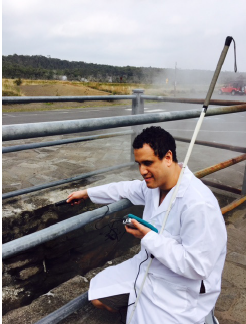
\includegraphics[width=1\linewidth]{fig1.png}
\end{figure}

There was a time when I was in high school chemistry class and I was prohibited from touching anything while a laboratory experiment was being conducted. This of course created a very hands-off learning experience for me, and frankly quite boring. I must say, at the end of my chemistry experience in high school, I did not like it very much. It was this mindset that carried with me into my under graduate studies at Purdue.

It was in this time of my life where I worked with a sighted assistant who acted as my eyes in the laboratory and described everything that was happening in the experiment. \textsuperscript{11} This approach is commonly used today, and it is beneficial for many reasons. Some of which fulfills the academic requirement, the student with the visual impairment has a minimal opportunity of getting injured in the class, and most importantly, the blind student is allowed to progress through their academic course of studies. However, in many cases, this continuation does not involve a STEM career path. The question is why?

How essential is a hands-on science learning experience tied to student interest? Educational research has found a direct link between student interest and hands-on science learning.\textsuperscript{12} This finding can safely be extended to the blind.\textsuperscript{13}

Through the efforts of organizations like Independence Science whose primary mission is to serve as a one stop shop for teachers of the blind and science faculty to provide an entire suite of products and services designed to empower the blind to have hands-on science learning experiences and to make them an integral part of any laboratory group.\textsuperscript{14 15} Further, it is the research interest of many of you today that will compliment and promote these efforts. Through these efforts of all of us here today will surely bring a revolution of opportunity to the blind in STEM education.

\end{large}
\clearpage
\section*{REFERENCES}\par 

\leftskip 0.25in
\parindent -0.25in 
1. Microsoft Encarta College Dictionary. St. Martin’s Press: New York, NY, 2001.

2. Wright, P. W. D.; Wright, P. D., Wrightslaw: IDEA 2004. Harbor House Law Press: Hartfield, VA, 2005.

3. Miner, D.; Nieman, R.; Swanson, A.; Woods, M., Teaching Chemistry to Students with Disabilities: A Manual for High Schools, Colleges, and Graduate Programs. 4th ed.; American Chemical Society Committee on Chemists with Disabilities: Washington, D.C., 2001.

4. Woods, M. a., Working Chemists with Disabilities: Expanding Opportunities in Science. American Chemical Society: Washington, D.C., 1996.

5. Margaret A. Browne, E. U. S. D. o. E. Letter of Resolution 2011. 

6. (a) Riccobono, M. A., The Spirit of the Journey: The Blind Driver Challenge and the Direction of Our Movement. \textit{Braille Monitor} \textbf{2011}, \textit{54} (8); (b) Riccobono, M. A., Driving Independence and Innovation through Imagination - The NFB Blind Driver Challenge. \textit{Braille Monitor} \textbf{2009}, \textit{52} (11).

7. (a) Mason, A., Mainstream Access to E-Books--What Works, What Doesn’t, and What Is Still Unclear. \textit{Braille Monitor} \textbf{2011}, \textit{54} (1); (b) Majerus, W., Access to Electronic Books, a Comparative Review. \textit{Braille Monitor} \textbf{2012}, \textit{55} (1).

8. Maurer, M., \textit{If Blindness Comes}. National Federation of the Blind: 2001.

9. Scadden, L. \textit{Current Status of People with Disabilities in STEM Education: A Personal Perspective}; Regional Alliance for Science, Engineering, \& Mathematics - Squared (RASEM2): Las Cruces, NM, 2005.

10. Jernigan, K., Blindness - Concepts and Misconceptions. \textit{Braille Monitor} \textbf{1965}, \textit{Aug. 1965}, 76-85.

11. Supalo, C., Techniques to Enhance Instructors’ Teaching Effectiveness with Chemistry Students Who Are Blind or Visually Impaired. \textit{J. Chem. Educ.} \textbf{2005}, \textit{82} (10), 1513-1518.

12. Piaget, J., \textit{Science of Education and the Psychology of the Child}. Orion Press: New York, NY, 1970.

13. Supalo, C. Teaching Chemistry and Other Sciences to Blind and Low-Vision Students Through Hands-On Learning Experiences in High School Science Laboratories. Pennsylvania State University, State College, PA, 2010.

14. Independence Science.

15. Mallouk, E. T. ILAB, Independent Laboratory Access for the Blind. (accessed November 1, 2012).
\clearpage
\begin{large}
\leftskip 0in
\parindent 0in 
\section*{BIOGRAPHICAL STATEMENT}

Dr. Cary Supalo received his P.h.D. from Penn State University in 2010. His research interest is in the area of promoting hands-on science learning experiences for blind and visually impaired students in science education. He graduated from Purdue University in 1999 with his Bachelor‘s degrees in chemistry and communications. He is an active member of the American Chemical Society‘s Chemists with Disabilities committee and serves on the National Federation of the Blind‘s Research and Development committee. He has been an active member of the Federation since he attended his first national convention in Dallas in 1993 and has attended every convention since. He has organized a number of hands-on science education workshops for blind children at NFB conventions since 2006 and has been involved in NFB Jernigan Institute‘s science education activities since the founding of the National Center for Blind Youth in Science. He currently serves as a consultant for Haverford College in Philadelphia and a visiting scientist at Purdue University in the Department of Chemistry. He is working on a teacher training manual for science educators on how to teach chemistry and other sciences in a hands-on way. He is coauthoring this publication with Dr. George M. Bodner at Purdue University. He oversees the development of new innovative text-to-speech technologies to empower the blind to have hands-on science learning experiences

\end{large}
\end{document}
